\problemname{Eagle attack}
\noindent
The squirrels and eagles have been at war since ancient times.
The Old Squirrel is a master of astrology and has predicted that the eagles will soon attempt one last attack on the Great Tree.
According to the Old Squirrel, a number of eagles will fly into the tree at high speed to make the whole tree shake, causing the squirrels to risk falling down.

The tree consists of $N - 1$ branches, which connects $N$ different points that we call \emph{nodes} (with the tree's trunk being node $1$).
Each branch in the tree thus connects two of these nodes.
The Old Squirrel has predicted which of the tree's $N$ nodes each of the eagles will crash into and at what speed.
He wants to know how much each node will shake during the attack to warn all the squirrels about the most dangerous nodes.
Unfortunately, the Old Squirrel is not as good at programming as he is at astrology, so he has hired you to calculate how much each node will shake during the attack.

When an eagle crashes with speed $v$ into node $u$, node $u$ begins to shake with strength $v$.
The shaking then spreads through the branches that extend from node $u$.
When the shaking reaches a certain node, it will spread through all the branches that meet at the new node, except the one the shaking came from.
The shaking strength spreads equally along these new branches, so if the shaking had strength $v$ and spreads along $k$ branches, the shaking traveling along the branches will have strength $\frac{v}{k}$.
This continues until the shaking eventually reaches nodes that have no other branches than the one from which the shaking came, where the shaking stops spreading.

You can assume that the shaking from a crash spreads through the entire tree and dissipates before the next eagle crashes.
For each of the nodes in the tree, the Old Squirrel wants to know the sum of all the shaking strengths that the node will be subjected to.

\section*{Input}
The first line contains the integer $N$ ($1 \le N \le 100,000$), the number of nodes in the tree.
The following $N-1$ lines each contain two integers $a$ and $b$ ($1 \le a, b \le N$), indicating that there is a branch between node $a$ and node $b$.

Next, there is a line with the integer $K$ ($1 \le K \le 100,000$), the number of eagles that will attack.
Finally, there are $K$ lines describing the eagles in the order they crash into the tree.
Each line contains two integers, the node $u$ ($1 \le u \le N$) where the eagle will crash and the eagle's speed $v$ ($1 \le v \le 10^9$).

\section*{Output}
Print one line for each node in the order $1$, $2$, $\dots$ with the sum of all shaking strengths that the node will be subjected to.
Your answer is considered correct if it has an absolute or relative error of at most $10^{-5}$.

\section*{Points}
Your solution will be tested on several test case groups.
To get the points for a group, it must pass all the test cases in the group.

\noindent
\begin{tabular}{| l | l | p{12cm} |}
  \hline
  \textbf{Group} & \textbf{Point value} & \textbf{Constraints} \\ \hline
  $1$    & $15$       &  The $i$th edge connects node $i$ and node $i+1$ (for all $1 \le i \le N-1$). \\ \hline 
  $2$    & $30$       &  $1 \le N,K \le 2000$ \\ \hline
  $3$    & $5$        &  $1 \le N \le 2000$ \\ \hline
  $4$    & $50$        &  No additional constraints. \\ \hline
\end{tabular}

\section*{Explanation of Sample 2}
\begin{figure}
  \centering
  \begin{minipage}{.5\textwidth}
    \centering
    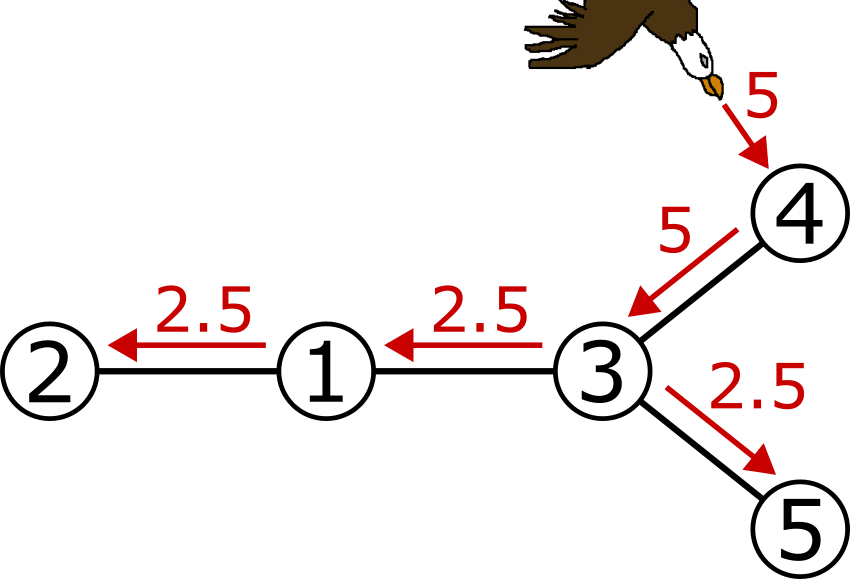
\includegraphics[width=0.8\textwidth]{a}
    \caption{First eagle.}
    \label{fig:test1}
  \end{minipage}%
  \begin{minipage}{.5\textwidth}
    \centering
    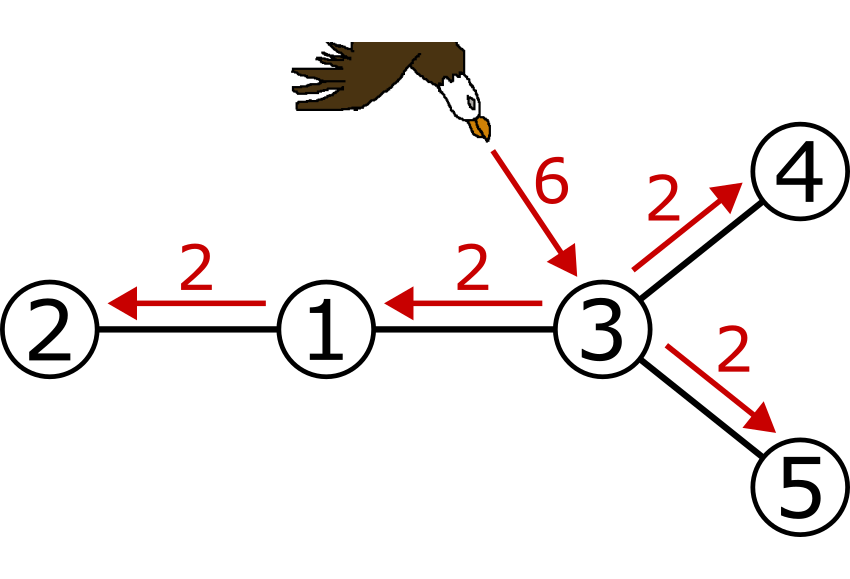
\includegraphics[width=0.8\textwidth]{b}
    \caption{Second eagle.}
    \label{fig:test2}
  \end{minipage}
\end{figure}

The first eagle crashes into node $4$ with a speed of $5$.
From node $4$, the shaking spreads only to node $3$ and from node $3$ to both nodes $1$ and $5$.
From node $5$, the shaking has nowhere to go, but from node $1$ it spreads to node $2$.

The second eagle crashes into node $3$ with a speed of $6$.
From node $3$, the shaking spreads to nodes $1$, $4$, and $5$.
The shaking in nodes $4$ and $5$ has nowhere to go, but the shaking in node $1$ spreads to node $2$.

To get the answers, the shaking values for each node are added together, for example, the answer is $2.5+2=4.5$ in node $1$ and $5+6=11$ in node $3$.
